% Created by tikzDevice version 0.6.2-92-0ad2792 on 2013-11-02 06:59:33
% !TEX encoding = UTF-8 Unicode
\documentclass[12pt, mainfont = Minion,     mainscale = 1.0, sansfont = Myriad,     sansscale = MatchLowercase, monofont = Consolas,   monoscale = MatchLowercase, mathfont = MinionMath, mathscale = 1.0]{mtikzfig}
\begin{document}

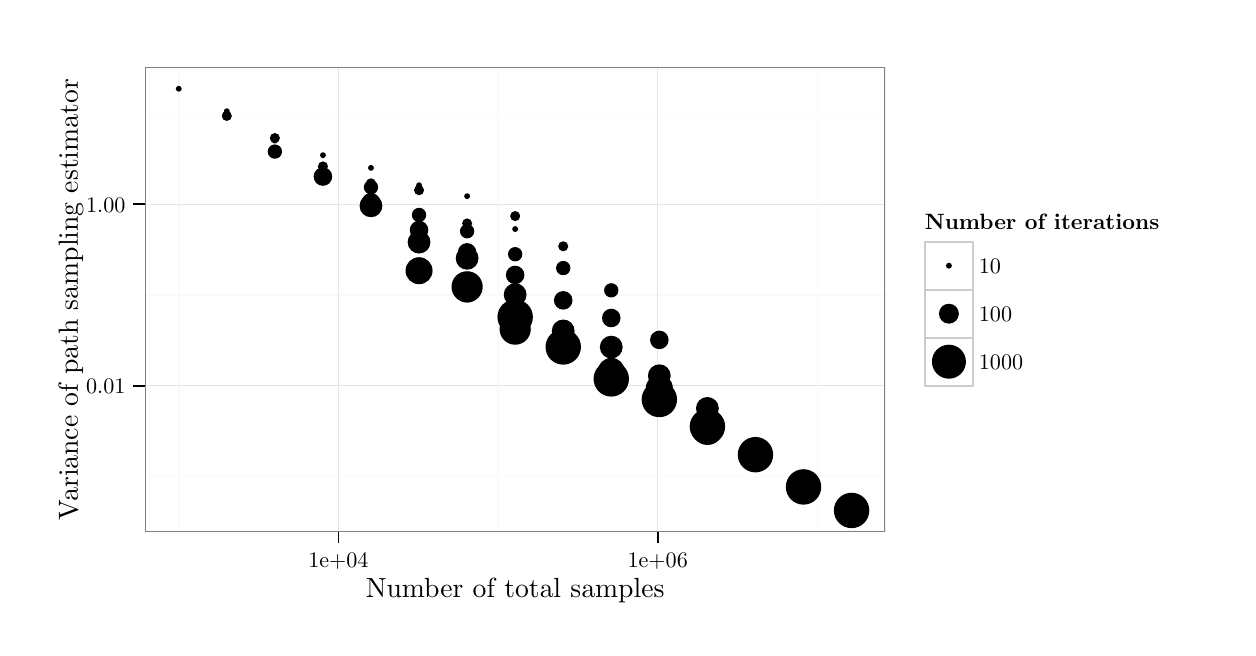
\begin{tikzpicture}[x=1pt,y=1pt]
\definecolor[named]{fillColor}{rgb}{1.00,1.00,1.00}
\path[use as bounding box,fill=fillColor,fill opacity=0.00] (0,0) rectangle (433.62,216.81);
\begin{scope}
\path[clip] (  0.00,  0.00) rectangle (433.62,216.81);
\definecolor[named]{drawColor}{rgb}{1.00,1.00,1.00}
\definecolor[named]{fillColor}{rgb}{1.00,1.00,1.00}

\path[draw=drawColor,line width= 0.6pt,line join=round,line cap=round,fill=fillColor] (  0.00,  0.00) rectangle (433.62,216.81);
\end{scope}
\begin{scope}
\path[clip] ( 42.43, 34.74) rectangle (309.87,202.36);
\definecolor[named]{fillColor}{rgb}{1.00,1.00,1.00}

\path[fill=fillColor] ( 42.43, 34.74) rectangle (309.87,202.36);
\definecolor[named]{drawColor}{rgb}{0.98,0.98,0.98}

\path[draw=drawColor,line width= 0.6pt,line join=round] ( 42.43, 54.67) --
	(309.87, 54.67);

\path[draw=drawColor,line width= 0.6pt,line join=round] ( 42.43,120.21) --
	(309.87,120.21);

\path[draw=drawColor,line width= 0.6pt,line join=round] ( 42.43,185.74) --
	(309.87,185.74);

\path[draw=drawColor,line width= 0.6pt,line join=round] ( 54.59, 34.74) --
	( 54.59,202.36);

\path[draw=drawColor,line width= 0.6pt,line join=round] (169.97, 34.74) --
	(169.97,202.36);

\path[draw=drawColor,line width= 0.6pt,line join=round] (285.35, 34.74) --
	(285.35,202.36);
\definecolor[named]{drawColor}{rgb}{0.90,0.90,0.90}

\path[draw=drawColor,line width= 0.2pt,line join=round] ( 42.43, 87.44) --
	(309.87, 87.44);

\path[draw=drawColor,line width= 0.2pt,line join=round] ( 42.43,152.98) --
	(309.87,152.98);

\path[draw=drawColor,line width= 0.2pt,line join=round] (112.28, 34.74) --
	(112.28,202.36);

\path[draw=drawColor,line width= 0.2pt,line join=round] (227.66, 34.74) --
	(227.66,202.36);
\definecolor[named]{fillColor}{rgb}{0.00,0.00,0.00}

\path[fill=fillColor] ( 54.59,194.74) circle (  1.07);

\path[fill=fillColor] ( 71.95,184.92) circle (  1.82);

\path[fill=fillColor] ( 89.32,172.03) circle (  2.59);

\path[fill=fillColor] (106.69,163.01) circle (  3.35);

\path[fill=fillColor] (124.05,152.43) circle (  4.12);

\path[fill=fillColor] (141.42,128.99) circle (  4.88);

\path[fill=fillColor] (158.79,123.16) circle (  5.64);

\path[fill=fillColor] (176.15,112.24) circle (  6.40);

\path[fill=fillColor] ( 71.95,186.62) circle (  1.07);

\path[fill=fillColor] ( 89.32,176.93) circle (  1.82);

\path[fill=fillColor] (106.69,163.63) circle (  2.59);

\path[fill=fillColor] (124.05,153.75) circle (  3.35);

\path[fill=fillColor] (141.42,139.31) circle (  4.12);

\path[fill=fillColor] (158.79,122.40) circle (  4.88);

\path[fill=fillColor] (176.15,107.88) circle (  5.64);

\path[fill=fillColor] (193.52,101.44) circle (  6.40);

\path[fill=fillColor] ( 89.32,176.01) circle (  1.07);

\path[fill=fillColor] (106.69,166.67) circle (  1.82);

\path[fill=fillColor] (124.05,159.14) circle (  2.59);

\path[fill=fillColor] (141.42,143.70) circle (  3.35);

\path[fill=fillColor] (158.79,133.47) circle (  4.12);

\path[fill=fillColor] (176.15,112.65) circle (  4.88);

\path[fill=fillColor] (193.52,100.95) circle (  5.64);

\path[fill=fillColor] (210.88, 89.90) circle (  6.40);

\path[fill=fillColor] (106.69,170.73) circle (  1.07);

\path[fill=fillColor] (124.05,160.57) circle (  1.82);

\path[fill=fillColor] (141.42,149.13) circle (  2.59);

\path[fill=fillColor] (158.79,135.62) circle (  3.35);

\path[fill=fillColor] (176.15,120.33) circle (  4.12);

\path[fill=fillColor] (193.52,100.42) circle (  4.88);

\path[fill=fillColor] (210.88, 90.48) circle (  5.64);

\path[fill=fillColor] (228.25, 82.46) circle (  6.40);

\path[fill=fillColor] (124.05,166.15) circle (  1.07);

\path[fill=fillColor] (141.42,158.07) circle (  1.82);

\path[fill=fillColor] (158.79,143.25) circle (  2.59);

\path[fill=fillColor] (176.15,127.45) circle (  3.35);

\path[fill=fillColor] (193.52,107.23) circle (  4.12);

\path[fill=fillColor] (210.88, 92.62) circle (  4.88);

\path[fill=fillColor] (228.25, 81.99) circle (  5.64);

\path[fill=fillColor] (245.62, 72.67) circle (  6.40);

\path[fill=fillColor] (141.42,159.86) circle (  1.07);

\path[fill=fillColor] (158.79,146.06) circle (  1.82);

\path[fill=fillColor] (176.15,134.95) circle (  2.59);

\path[fill=fillColor] (193.52,118.28) circle (  3.35);

\path[fill=fillColor] (210.88,101.38) circle (  4.12);

\path[fill=fillColor] (228.25, 86.59) circle (  4.88);

\path[fill=fillColor] (245.62, 71.66) circle (  5.64);

\path[fill=fillColor] (262.98, 62.51) circle (  6.40);

\path[fill=fillColor] (158.79,155.91) circle (  1.07);

\path[fill=fillColor] (176.15,148.73) circle (  1.82);

\path[fill=fillColor] (193.52,129.94) circle (  2.59);

\path[fill=fillColor] (210.88,111.90) circle (  3.35);

\path[fill=fillColor] (228.25, 91.03) circle (  4.12);

\path[fill=fillColor] (245.62, 74.85) circle (  4.88);

\path[fill=fillColor] (262.98, 61.94) circle (  5.64);

\path[fill=fillColor] (280.35, 50.86) circle (  6.40);

\path[fill=fillColor] (176.15,144.04) circle (  1.07);

\path[fill=fillColor] (193.52,137.81) circle (  1.82);

\path[fill=fillColor] (210.88,121.90) circle (  2.59);

\path[fill=fillColor] (228.25,103.99) circle (  3.35);

\path[fill=fillColor] (245.62, 79.23) circle (  4.12);

\path[fill=fillColor] (262.98, 62.57) circle (  4.88);

\path[fill=fillColor] (280.35, 50.50) circle (  5.64);

\path[fill=fillColor] (297.72, 42.36) circle (  6.40);
\definecolor[named]{drawColor}{rgb}{0.50,0.50,0.50}

\path[draw=drawColor,line width= 0.6pt,line join=round,line cap=round] ( 42.43, 34.74) rectangle (309.87,202.36);
\end{scope}
\begin{scope}
\path[clip] (  0.00,  0.00) rectangle (433.62,216.81);
\definecolor[named]{drawColor}{rgb}{0.00,0.00,0.00}

\node[text=drawColor,anchor=base east,inner sep=0pt, outer sep=0pt, scale=  0.80] at ( 35.32, 84.51) {0.01};

\node[text=drawColor,anchor=base east,inner sep=0pt, outer sep=0pt, scale=  0.80] at ( 35.32,150.05) {1.00};
\end{scope}
\begin{scope}
\path[clip] (  0.00,  0.00) rectangle (433.62,216.81);
\definecolor[named]{drawColor}{rgb}{0.00,0.00,0.00}

\path[draw=drawColor,line width= 0.6pt,line join=round] ( 38.16, 87.44) --
	( 42.43, 87.44);

\path[draw=drawColor,line width= 0.6pt,line join=round] ( 38.16,152.98) --
	( 42.43,152.98);
\end{scope}
\begin{scope}
\path[clip] (  0.00,  0.00) rectangle (433.62,216.81);
\definecolor[named]{drawColor}{rgb}{0.00,0.00,0.00}

\path[draw=drawColor,line width= 0.6pt,line join=round] (112.28, 30.47) --
	(112.28, 34.74);

\path[draw=drawColor,line width= 0.6pt,line join=round] (227.66, 30.47) --
	(227.66, 34.74);
\end{scope}
\begin{scope}
\path[clip] (  0.00,  0.00) rectangle (433.62,216.81);
\definecolor[named]{drawColor}{rgb}{0.00,0.00,0.00}

\node[text=drawColor,anchor=base,inner sep=0pt, outer sep=0pt, scale=  0.80] at (112.28, 21.77) {1e+04};

\node[text=drawColor,anchor=base,inner sep=0pt, outer sep=0pt, scale=  0.80] at (227.66, 21.77) {1e+06};
\end{scope}
\begin{scope}
\path[clip] (  0.00,  0.00) rectangle (433.62,216.81);
\definecolor[named]{drawColor}{rgb}{0.00,0.00,0.00}

\node[text=drawColor,anchor=base,inner sep=0pt, outer sep=0pt, scale=  1.00] at (176.15, 10.84) {Number of total samples};
\end{scope}
\begin{scope}
\path[clip] (  0.00,  0.00) rectangle (433.62,216.81);
\definecolor[named]{drawColor}{rgb}{0.00,0.00,0.00}

\node[text=drawColor,rotate= 90.00,anchor=base,inner sep=0pt, outer sep=0pt, scale=  1.00] at ( 18.16,118.55) {Variance of path sampling estimator};
\end{scope}
\begin{scope}
\path[clip] (  0.00,  0.00) rectangle (433.62,216.81);
\definecolor[named]{fillColor}{rgb}{1.00,1.00,1.00}

\path[fill=fillColor] (319.95, 83.17) rectangle (409.09,153.93);
\end{scope}
\begin{scope}
\path[clip] (  0.00,  0.00) rectangle (433.62,216.81);
\definecolor[named]{drawColor}{rgb}{0.00,0.00,0.00}

\node[text=drawColor,anchor=base west,inner sep=0pt, outer sep=0pt, scale=  0.80] at (324.21,143.81) {\bfseries Number of iterations};
\end{scope}
\begin{scope}
\path[clip] (  0.00,  0.00) rectangle (433.62,216.81);
\definecolor[named]{drawColor}{rgb}{0.80,0.80,0.80}
\definecolor[named]{fillColor}{rgb}{1.00,1.00,1.00}

\path[draw=drawColor,line width= 0.6pt,line join=round,line cap=round,fill=fillColor] (324.21,122.13) rectangle (341.56,139.47);
\end{scope}
\begin{scope}
\path[clip] (  0.00,  0.00) rectangle (433.62,216.81);
\definecolor[named]{fillColor}{rgb}{0.00,0.00,0.00}

\path[fill=fillColor] (332.89,130.80) circle (  1.07);
\end{scope}
\begin{scope}
\path[clip] (  0.00,  0.00) rectangle (433.62,216.81);
\definecolor[named]{drawColor}{rgb}{0.80,0.80,0.80}
\definecolor[named]{fillColor}{rgb}{1.00,1.00,1.00}

\path[draw=drawColor,line width= 0.6pt,line join=round,line cap=round,fill=fillColor] (324.21,104.78) rectangle (341.56,122.13);
\end{scope}
\begin{scope}
\path[clip] (  0.00,  0.00) rectangle (433.62,216.81);
\definecolor[named]{fillColor}{rgb}{0.00,0.00,0.00}

\path[fill=fillColor] (332.89,113.45) circle (  3.60);
\end{scope}
\begin{scope}
\path[clip] (  0.00,  0.00) rectangle (433.62,216.81);
\definecolor[named]{drawColor}{rgb}{0.80,0.80,0.80}
\definecolor[named]{fillColor}{rgb}{1.00,1.00,1.00}

\path[draw=drawColor,line width= 0.6pt,line join=round,line cap=round,fill=fillColor] (324.21, 87.44) rectangle (341.56,104.78);
\end{scope}
\begin{scope}
\path[clip] (  0.00,  0.00) rectangle (433.62,216.81);
\definecolor[named]{fillColor}{rgb}{0.00,0.00,0.00}

\path[fill=fillColor] (332.89, 96.11) circle (  6.14);
\end{scope}
\begin{scope}
\path[clip] (  0.00,  0.00) rectangle (433.62,216.81);
\definecolor[named]{drawColor}{rgb}{0.00,0.00,0.00}

\node[text=drawColor,anchor=base west,inner sep=0pt, outer sep=0pt, scale=  0.80] at (343.73,127.87) {10};
\end{scope}
\begin{scope}
\path[clip] (  0.00,  0.00) rectangle (433.62,216.81);
\definecolor[named]{drawColor}{rgb}{0.00,0.00,0.00}

\node[text=drawColor,anchor=base west,inner sep=0pt, outer sep=0pt, scale=  0.80] at (343.73,110.53) {100};
\end{scope}
\begin{scope}
\path[clip] (  0.00,  0.00) rectangle (433.62,216.81);
\definecolor[named]{drawColor}{rgb}{0.00,0.00,0.00}

\node[text=drawColor,anchor=base west,inner sep=0pt, outer sep=0pt, scale=  0.80] at (343.73, 93.18) {1000};
\end{scope}
\end{tikzpicture}

\end{document}
